%%
%% This is file `cescgsmpl.tex',
%% generated with the docstrip utility.
%%
%% The original source files were:
%%
%% cescg.dtx  (with options: `sample')
%% 
%% IMPORTANT NOTICE:
%% 
%% For the copyright see the source file.
%% 
%% Any modified versions of this file must be renamed
%% with new filenames distinct from cescgsmpl.tex.
%% 
%% For distribution of the original source see the terms
%% for copying and modification in the file cescg.dtx.
%% 
%% This generated file may be distributed as long as the
%% original source files, as listed above, are part of the
%% same distribution. (The sources need not necessarily be
%% in the same archive or directory.)
%% Copyright (c) 1999, 2005
%%               Institute of Computer Graphics and Algorithms
%%               TU Vienna, Austria
%% Based on the LaTeX2e document class SCCG
%% Copyright (C) 1999 Pavel Chalmoviansky
%%                    Katedra geometrie
%%                    Faculty of Mathematics and Physics
%%                    Comenius University, Bratislava
%%                    chalmo@fmph.uniba.sk
%%
%% This file is distributed in the hope that it will be useful,
%% but WITHOUT ANY WARRANTY; without even the implied warranty of
%% MERCHANTABILITY or FITNESS FOR A PARTICULAR PURPOSE.
%%
%% \CharacterTable
%%  {Upper-case    \A\B\C\D\E\F\G\H\I\J\K\L\M\N\O\P\Q\R\S\T\U\V\W\X\Y\Z
%%   Lower-case    \a\b\c\d\e\f\g\h\i\j\k\l\m\n\o\p\q\r\s\t\u\v\w\x\y\z
%%   Digits        \0\1\2\3\4\5\6\7\8\9
%%   Exclamation   \!     Double quote  \"     Hash (number) \#
%%   Dollar        \$     Percent       \%     Ampersand     \&
%%   Acute accent  \'     Left paren    \(     Right paren   \)
%%   Asterisk      \*     Plus          \+     Comma         \,
%%   Minus         \-     Point         \.     Solidus       \/
%%   Colon         \:     Semicolon     \;     Less than     \<
%%   Equals        \=     Greater than  \>     Question mark \?
%%   Commercial at \@     Left bracket  \[     Backslash     \\
%%   Right bracket \]     Circumflex    \^     Underscore    \_
%%   Grave accent  \`     Left brace    \{     Vertical bar  \|
%%   Right brace   \}     Tilde         \~}
%%
\ProvidesFile{cescgsmpl.tex}
            [2005/11/29 v0.1.4
 CESCG proceedings sample file]
 %%% The document class command loads the CESCG class and sets the basic
 %%%  options.  See the user's guide for more options and their meaning.


\documentclass{cescg}[2005/11/12] % Use this for your submission and the final paper
 %%% Use e.g. this package to include figures via \includegraphics[options]{filename}.
 %%% If you don't have it in your latex installation, complain to your
 %%% sysadmin that he's not doing his job.
\usepackage{graphicx}
 %%% The following packages are somewhat system and installation dependent, and may not work
 %%% on some systems.
 %%% If you use pdfLaTeX on Windows (part of MiKTeX), you may use package epstopdf to automatically
 %%% convert eps files to pdf. Use this line:
 %\usepackage{epstopdf}
 %%% Linux users may have to call epstopdf on the command line or configure a Makefile appropriately.

 %%% If you know how to create bounding boxes for png and jpg files, you can uncomment this
 %%% to include png files etc. directly.
 %%% For example bmeps -b myfigure.png >myfigure.bb will do the trick in Windows.
 %%% Also, dvips needs the option "-I c3r8f" to be able to convert the bitmaps.
 %%% See the bmeps faq for more info: http://bmeps.sourceforge.net/faq.html
 %\ifx\pdfoutput\undefined \DeclareGraphicsExtensions{.eps,.png,.gif,.jpg} \fi

 %%% Now we set the fields for the title block and cover sheet
 %%% See the user's guide for more information on these items

 %% Title, author(s), and affiliation
 %%  Note that we have included both individual affiliations for each author
 %%   within the author block, as well as a common affiliation.  Only one
 %%   of these is necessary.
 %%  Footnotes to items in the title block should be created with the \thanks
 %%   command.
\title{Rapid Modeling of Geology}
\author{Morten Bendiksen\thanks{morten.bendiksen@gmail.com}}
\supervisor{Endre M. Lidal\thanks{endre@mail.com}} % TODO add emails
\affiliation{Institute of Informatics\\
             University of Bergen}

 %% Keywords of paper
\keywords{Rapid Modeling, SBIM, Geology}
 %%% Begin the paper
\begin{document}

 %%% Create the title block
\maketitle

 %%% The abstract
\begin{abstract}
 Drawing three dimensional models of geological phenomena is today a process requiring training in specific programs that can be very time consuming. For illustration and communication of geological concepts, geologists therefore often limit themselves to drawing on paper or to two dimensional drawing applications.

I propose an approach for making rapid geologic illustrations in 3D. The novel idea for the approach consists of sketch based input on a cube in order to create a layered geological structure. Further details can be added to the layers by sketching geological concepts such as rivers, mountains and valleys. Sedimentary deposits can be created through a procedural modeling approach that employs a volume preserving diffusion algorithm to simulate the flow of depositional material on top of the terrain. Awareness of the geologic domain enables a sparse amount of input strokes to be interpreted into geological structures.

Results show that the proposed approach can be used with success to model geological layers. Compared with a 2D sketch, the creation of a 3D geometry on a computer gives advantages such as perspective control, ease of making changes to the model, etc. The approach shows great promise and can be useful in many situations. A program based on the proposed approach could become a standard way for geologists to draw their illustrations.
\end{abstract}

 %%% Keywords

\keywordlist

 %%% The main text
\section{Introduction}

\begin{figure}
 \centering
 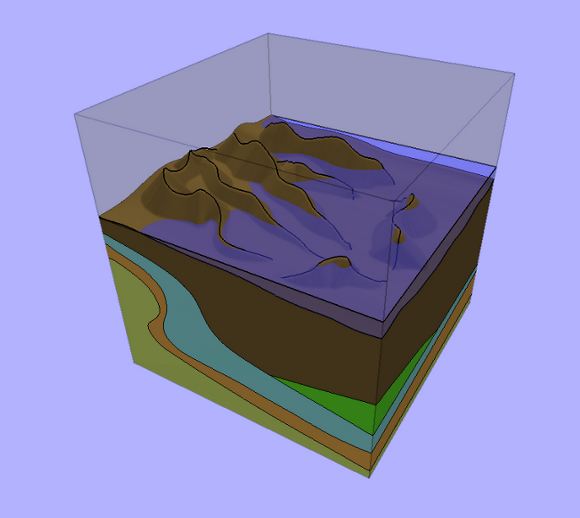
\includegraphics[width=0.7\linewidth]{approachSketch.png}
 % TODO insert reference
 \caption{A typical sketch made with the proposed approach. }
 \label{fig:approachSketch}
\end{figure}

% 
% \begin{figure}[b]
%  \centering
%  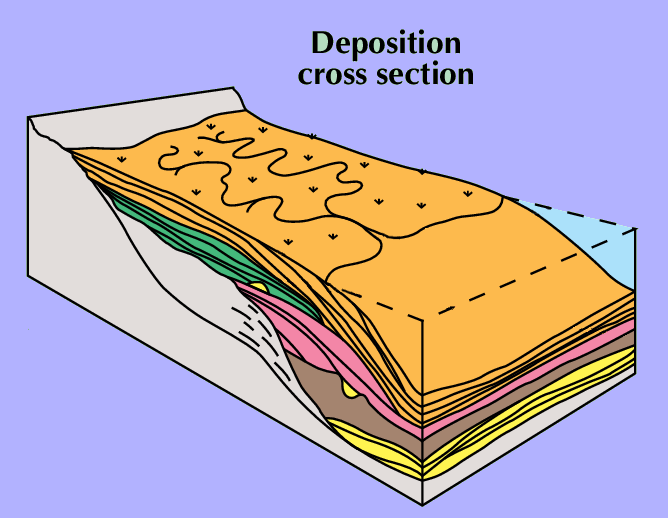
\includegraphics[width=0.7\linewidth]{strataSketch.png}
%  % TODO insert reference
%  \caption{A typical sketch from a earth science paper. }
%  \label{fig:strataSketch}
% \end{figure}
It is a common practice to make sketched geological models by hand on either paper or computer. These sketches are used in both professional and educational settings, and facilitate communication and understanding. Geologic phenomena are four dimensional in nature since they occur over time in the three spatial dimensions. There are many techniques and standards for illustrating these phenomena in a two dimensional drawing. One can for example sketch three dimensional phenomena by using perspective drawing techniques, but the model is still confined to the 2D nature of the medium. These techniques and standards can also be limiting  as they require significant time and training to master and understand. Before I started working on this project a problem was identified; there did not exist any tools aimed at helping geologists sketch 3D models for illustration purposes. On the computer it is already possible to make 3D models in traditional modeling approaches. However, existing tools are often complex, aimed 
at creating advanced and detailed models, and usually requires training to understand and use. It is from this background that the goal of this project was formed. 



The goal of this project is to enable the rapid creation of 3D models of geologic structures by creating an approach that lets geologists quickly specify input in an intuitive way that is easy to learn. The model will be used for illustrative purposes to facilitate communication between geologists by letting them create sketched models quicker, help lecturers explain concepts to students by creating models that can be changed interactively, and reduce the need for artistic skills and long training for students to master illustration techniques. The study of sedimentary layer structures and the processes that deform such layers are perhaps the fields of study that has resulted in the most knowledge about the history of the Earth. I concentrate most effort around the creation of rapid modeling techniques for geological layer structures. The aim is to create an approach for the creation of such structures.

\section{Background}
The geologic understanding for this project was gained from reading the book ``Geologi, Stein, mineraler, fossiler og olje'', by Haakon Fossen \cite{fossen2008geologi}. For reference and technical background in the field of computer graphics the book ``Real Time Rendering'' \cite{moller2008real} has been used.  The book ``Curves and surfaces for CAGD: a practical guide'' \cite{farin2001curves} was used to understand curve and surface theory. 

Geology is a complex science, and this explains why there are so many subfields within geology. Of most interest to this project: Geomorphology is the study of landforms and the processes that shape the surface of the Earth. Sedimentology is about how particles are transported, where they are deposited and how they are compressed into rock. Structural geology is the study of how the rock layers and crust is deformed by various movements. Tectonics is closely related to Structural geology and describes the movement of Earth plates and how that causes the formation of mountain ranges and basins.



In geology, models are used for understanding and communicating about phenomena relating to the structure of the Earth and how it changes over time. At the first international conference for 3-D geoscientific modelling, held in 1989, Dr Brian Kelk defined the requirements for subsurface characterisation and modelling:
‘‘The industry requires a system for interactive creation
of spatial and spatio-temporal models of the physical
nature of portions of the Earth’s crust. i.e. the
capability to effectively model and visualise:
\begin{itemize}
 \item Geometry of rock- and time-stratigraphic units
 \item Spatial and temporal relationships between geo-objects
 \item Variation in internal composition of geo-objects
 \item Displacements or distortions by tectonic forces
 \item Fluid flow through rock units’’ \cite{turner1992three}
\end{itemize}

Traditional CAD systems have several problems when used to make geological models (Turner et al. \cite{turner2006challenges}). There have been attempts at using such system to create geological models (Kelk and Challen \cite{kelk1992experiments}). Such experiments have shown some problems in using standard CAD systems for geological modeling. The reason for this is the characteristics of geological objects. As Caumron et al. \cite{caumon2009surface} identify these include: complex geometry and topology, scale dependency and hierarchical relationships, indistinct boundaries defined by complex spatial variations and the intrinsic property heterogeneity and anisotropy of most subsurface features. The gOcad tool decscribed by Mallet \cite{mallet1992gocad}, however, has been developed to make a CAD approach for geomodeling, by basing the modeling on a new interpolation method called ``Discrete Smooth Interpolation''. The geometry is defined by bridging together a set of nodes with a location is 3D space and with 
physical properties attached to these nodes.

A realistic geological scenario will follow certain constraints.  Caumron et al. gives rules for modeling that define boundaries between layers. For example, geological objects have a spacial continuity such that abrupt changes of normal orientation are not common. This is relevant for the creation of layers in the approach I propose, as it allows the use of smooth curves to represent layers. They also describe  the typical process of creating a structural model. The modeling usually starts with fault modeling, then the connection between fault surfaces is defined. Finally horizons are modeled. If the fault structure is very complex, it is normal to start with horizon definition and introduce the faults after.

Natali et al. explores different modeling techniques in their recent survey paper \cite{natali2013modeling}. They describe a data-oriented taxonomy where modeling is divided into three different scenarios, one data-free, one sparse-data, and one dense-data. Natali et al. also show how geological modeling trends are approaching modeling methods that have been developed in computer graphics and give an in-depth description of selected methods that can be applied for geological modeling. The sparse-data and dense-data scenario occurs when there is geologically measured data available and used as input for a modeling approach. In this scenario there exists many approaches aimed at geologic use. The data-free scenario on the contrary has no ground truth information and relies entirely on procedural and/or geometric modeling. Not many approaches for input aimed specifically at geology exists in this scenario, but relevant techniques from other fields exist. In this thesis the approach described is a data-free 
scenario, since the idea is to create a sketching tool. However, some approaches from the sparse and dense-data scenarios are also relevant as the user sometimes will guide the interpretation of the input data to varying degrees. 

The data sparse scenario is the most common in the geosciences and is most often the result of borehole data collection. In such situations the data points are spread around and need to be interpolated, which is relevant for the approach I propose. The main interpolation methods are the B-Spline method, inverse distance method, Kriging method, and discrete smooth interpolation method \cite{mallet1992discrete, mallet1997discrete}. Interpolation methods are interesting in regards to the approach I propose as they might be used to interpolate horizons from the sketched curves for horizon creation. 

The data dense scenario is usually the case when data from seismic surveys is available. Here the problem is how to display the huge amounts of data, and how to interpret them to make a model of the structures present. Approaches that aim at making the interpretation process easier and quicker have emerged in recent years. Patel et al. describe techniques for rapid horizon extraction from seismic data in both 2D \cite{patel2008seismic} and 3D \cite{patel2010seismic}. Amorim et al. \cite{amorim2012sketch} have an interesting approach that allows sketching directly over the raw seismic reflection volume and its derived data to help build the structural model of the subsurface. This helps the expert in interpreting and and building a structural framework for a reservoir by using a sketch-based input for helping in the interpretation process.

Many existing tools are based on the assumption that there is extensive data available and that geologists will have a lot of time developing a model of the area of interest. Several tools exist for modeling, displaying, editing and automatically calculate parameters for geological modeling.  Petrel \cite{petrel} is an example of a commercial program for geologic modeling that is in use. Most of such existing tools rely on an intensive work flow, and are based on interpreting data gathered from seismic surveys or bore hole data. The modeling is done either automatically, or semi-automatically by letting the user indicate various parameters and alter the suggested model manually. Sometimes up to a year is spent on developing such models. Recently a need for rapid developments of geologic prospects have been identified. A lot of techniques have therefore been taken from other fields that model terrain, such as the video games industry and movie industry \cite{natali2013modeling}.

 Procedural generation is a standard way to generate terrains. This usually happens in one of three ways: fractal landscape modeling, physical erosion simulation and synthesis of terrain from images or sample terrain. Before Olsen \cite{olsen2004realtime} fractal noise was mostly used to create terrain surfaces, because of computer limitations on simulating erosion processes. Olsen proposed a synthesized fractal terrain and applies an erosion algorithm on that. The representation is a 2D height-map. Hnaidi et al. \cite{hnaidi2010feature} generate terrain that is constrained by a set of curves that characterize the features of the landscape. The ability to make realistic looking landscapes could be interesting in a rapid sketching tool, as the generated landscape is constrained by curves that could be input by sketching.
 
 
\begin{figure}
 \centering
 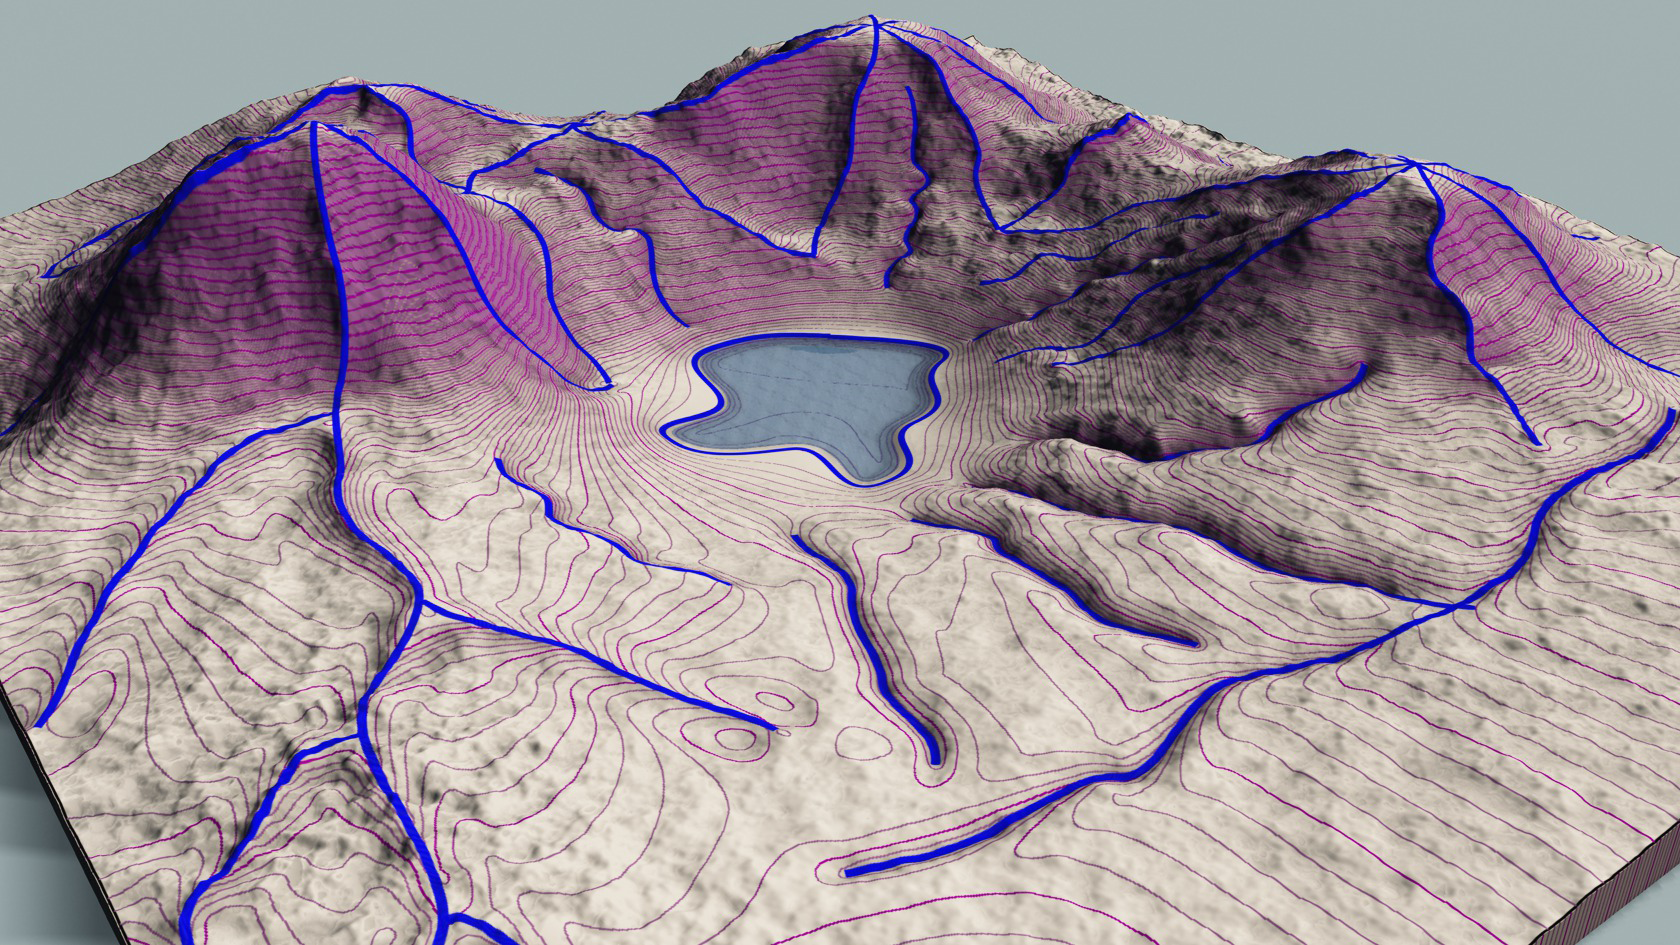
\includegraphics[width=0.5\textwidth]{thesis/related/hnaidi.png}
 \caption{Terrain generation by Hnaidi et al. \cite{hnaidi2010feature}. }
 \label{fig:hnaidi}
\end{figure}

 
 A method for eroding terrain is described by Benes et al. \cite{benes2001layered} where a concise voxel representation is created and then eroded by thermal weathering simulation. The representation allows for caves and hole structures. The same authors also propose a method for procedural modeling of terrain by hydraulic erosion \cite{benevs2002visual}. Stava et al. \cite{vst2008interactive} employ an interactive physics based hydraulic erosion. The user interacts during the generation of the terrain. These erosion techniques could be applied in the approach I propose as a way to make more realistic horizon surfaces. Erosion could also be used to simulate material transportation and deposits creation, rivers, etc.
 
 Peytavie et al. \cite{peytavie2009procedural} propose a way to model and render rock piles and stones which are found in most landscapes without any computationally demanding physically-based simulation. Peytavie et al. also have proposed a framework for representing complex terrains with such features as overhangs, arches and caves and including different materials such as sand and rocks \cite{peytavie2009arches}. This is done by a discrete volumetric representation with different kinds of material and an implicit representation for the modelling and reconstruction of the model. To allow more complex structures in sketches, such a representation could be useful, while rock piles might be useful to illustrate avalanches or other geological phenomena involving loose rocks.

\begin{figure}
 \centering
 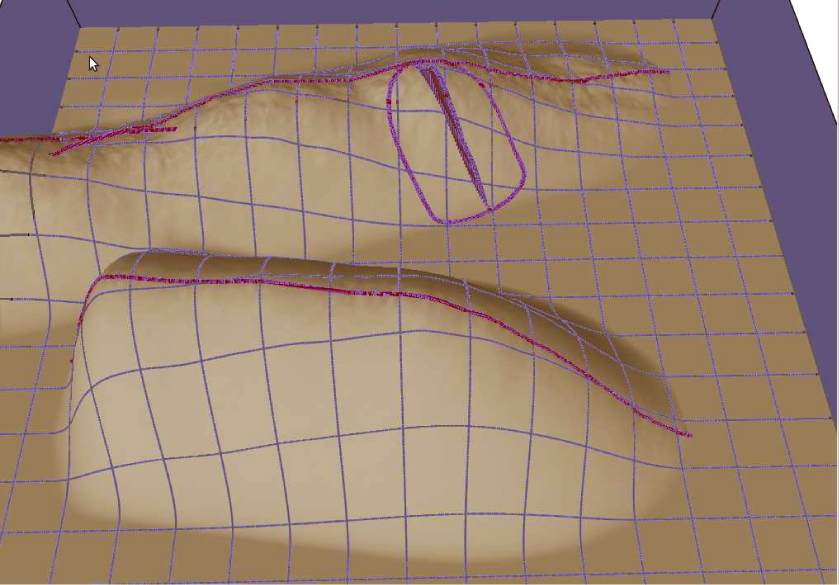
\includegraphics[width=0.4\textwidth]{thesis/related/tasse1.png}
 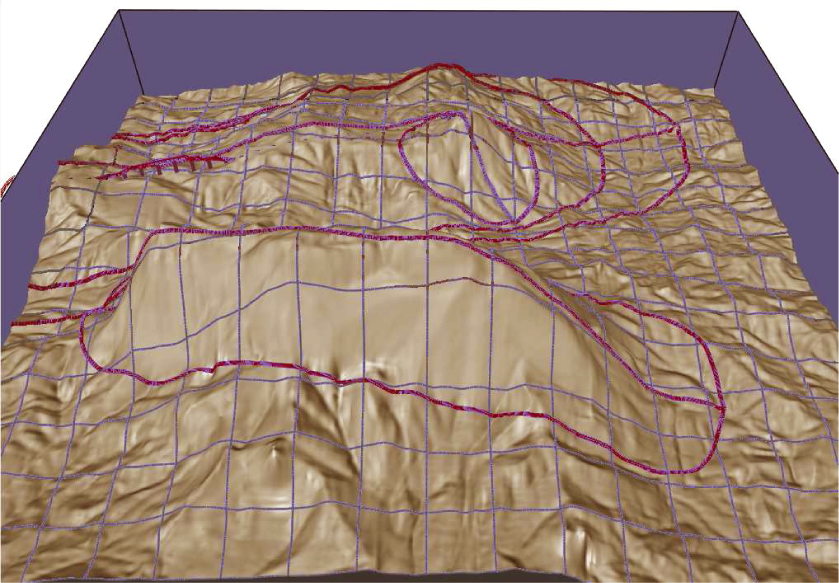
\includegraphics[width=0.4\textwidth]{thesis/related/tasse2.png}
 \caption{The terrain syntesis proposed by Tasse et al. \cite{tasse2012enhanced}. Left: user sketched curves. Right: final result. }
 \label{fig:tasse}
\end{figure}

 
 
Tasse et al. \cite{tasse2012enhanced} propose a texture-based terrain synthesis framework controllable by
a terrain sketching interface. They enhance the realism of the generated landscapes by using a novel patch merging
method that reduces boundary artifacts caused by overlapping terrain patches. The high computational cost of texture
synthesis is reduced with a parallel implementation on graphics hardware. This approach could also prove useful to create more realistic surfaces.


Natali et al. \cite{natalirapid} describe an approach where the user sketches the boundaries of geological layers. Then the user can sketch folding and faulting operations, and thus create many different scenarios. The input in this approach is restricted to making conceptually 2D sketches, allthough the visualization is in 3D. Projecting drawings on the 3D structure can however give some more information and context to the 3D geometry. The techniques for texturing that they describe makes their sketches carry a lot of expressive power of the internal structure of specific layers. The painting of details on surfaces also opens for many illustration purposes. This approach has been developed in parallel to the approach I propose. As far as I know, this is the only sketch based approach to modeling subsurface geological layers in 3D without measured data other than the one described in this thesis. However, Lidal et al. \cite{lidal2012geological} present Geological Storytelling, a novel graphical approach for 
performing and presenting rapid and expressive geomodeling of a multitude of model variations in 2D that handles sketching processed over time. This approach allows the user to sketch,  play back, and compare geological events as he believes they might have occurred over time.

\begin{figure}
 
 \centering
    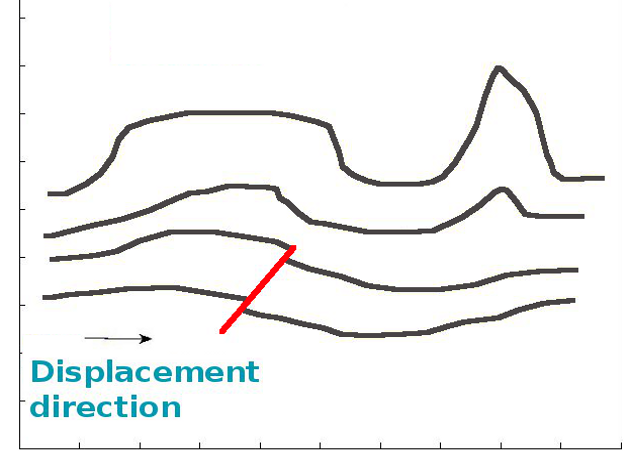
\includegraphics[width=0.3\textwidth]{thesis/related/natali1.png}
    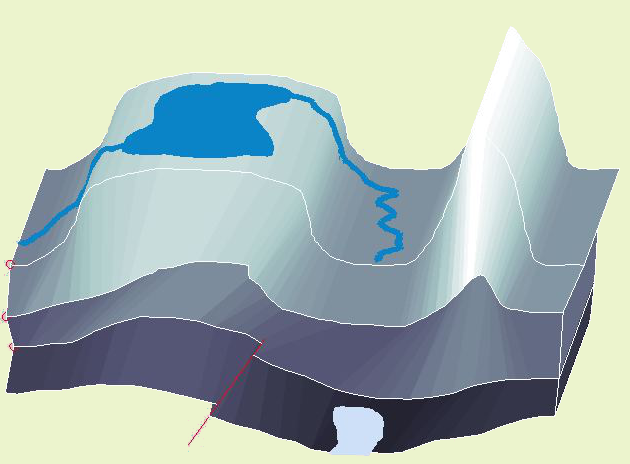
\includegraphics[width=0.3\textwidth]{thesis/related/natali2.png}
    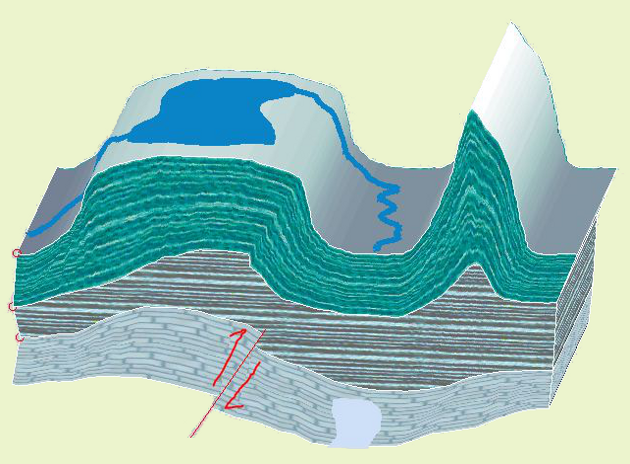
\includegraphics[width=0.3\textwidth]{thesis/related/natali3.png}
  \caption{The proposed interface by Natali et al. \cite{natalirapid}.  }
  \label{fig:nataliRapid}
\end{figure}


Cockett's Visual Geology \cite{Cockett:Online} and Jessell's Noddy \cite{jessell1981noddy} are two geologic modeling tools designed for educational purposes that allow rapid building of geological layer structures by user input of parameters. Visual Geology lets the user specify how many layers she wants and their thickness, and then apply various functions such as a fault line and its angle, a folding phenomenon and its angle, wave frequency etc. The basis for Noddy is the ability to construct a complex geological history as a succession of relatively simple structural, sedimentary and igneous events similarly to Visual Geometry, which allows the user to rapidly create models and then calculate resulting gravity and magnetic fields. Both of these are based on parameterized procedural methodologies.

\begin{figure}
\centering
 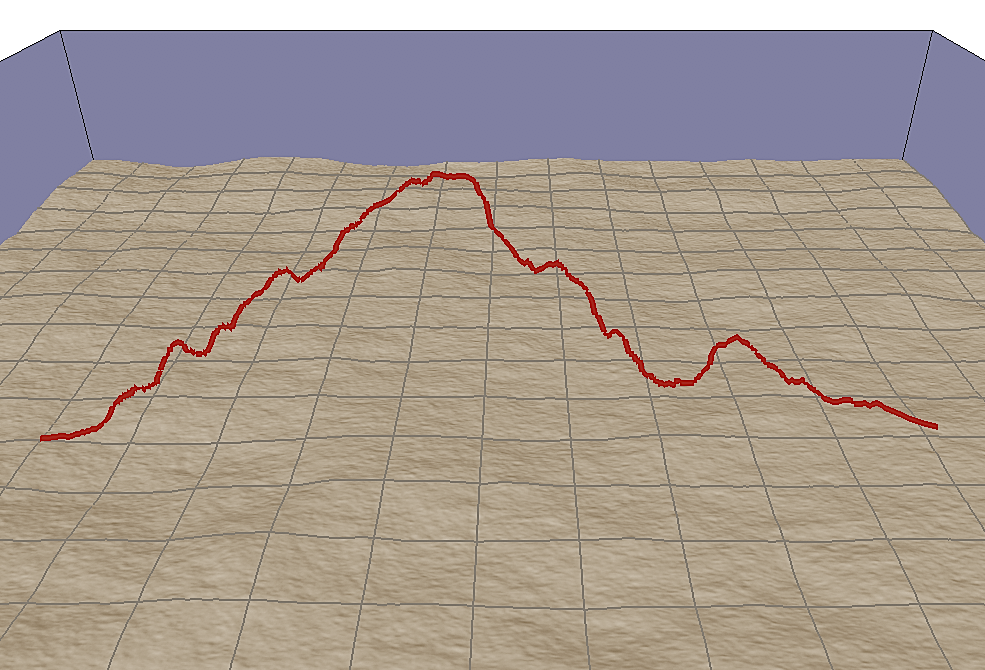
\includegraphics[width=0.4\linewidth]{thesis/related/img-001.png}
 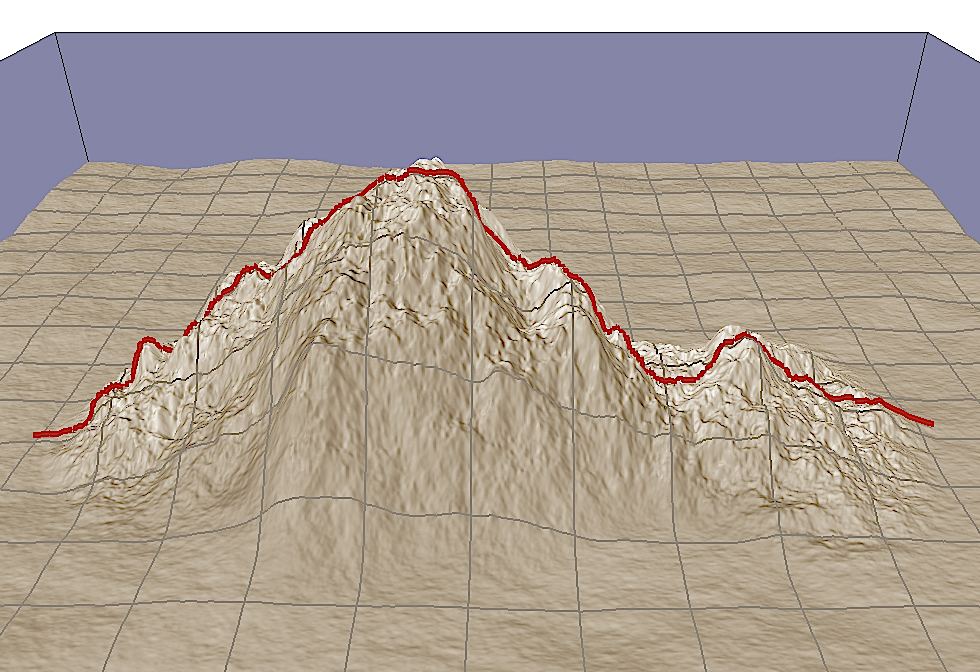
\includegraphics[width=0.4\linewidth]{thesis/related/img-002.png}
 \caption{The terrain sketching approach from Gain et al. \cite{Gain:2009:TS:1507149.1507155}. }
 \label{fig:gain}
\end{figure}


There exists several approaches for sketching terrain, which are applicable to geology. Harold is an early example of a sketch based system that incorporates methods for sketching terrain, made by Cohen et al. \cite{cohen2000harold}. In Harold, the user can sketch hills on the terrain by simple strokes that start and end on the terrain. The terrain is then warped to try and match the stroke. Watanabe et al.  \cite{Watanabe:2004:SIT:1186415.1186500} made a further development of this, where the shape of the stroke also influences the width of hills that are generated, making for more natural looking hills. They also incorporated noise on top of the generated terrain to make the visualization more realistic. Gain et al. \cite{Gain:2009:TS:1507149.1507155} later improved further on this by allowing the user to sketch the width of the hill and change the baseline along wich this hill runs. The approach by Gain et al. can be seen in Figure \ref{fig:gain}. To achieve real-time terrain creation Bernhardt et al. 
combine CPU and GPU processing in their sketch-based approach for generating and displaying complex and high-resolution terrains. The user can see the terrain changing as she is sketching. De Carpentier combine brushing and procedural terrain creation \cite{de2009interactive}. These terrain sketching techniques are all interesting in enabling sketching of terrain features like mountains. The ridge sketching in particular is inspired by all these papers on terrain sketching.

\begin{figure}
\centering
 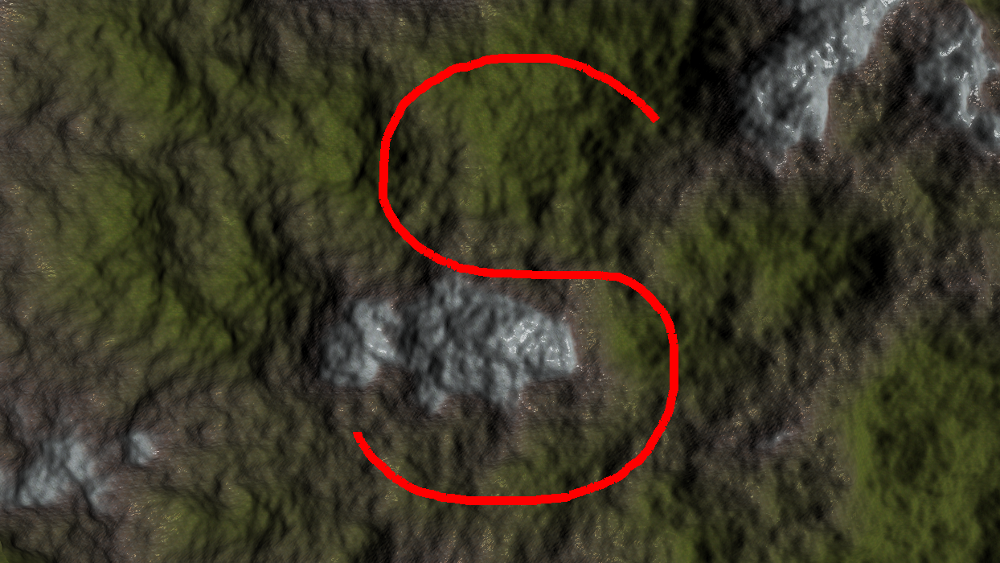
\includegraphics[width=0.4\linewidth]{thesis/related/applegate.png}
 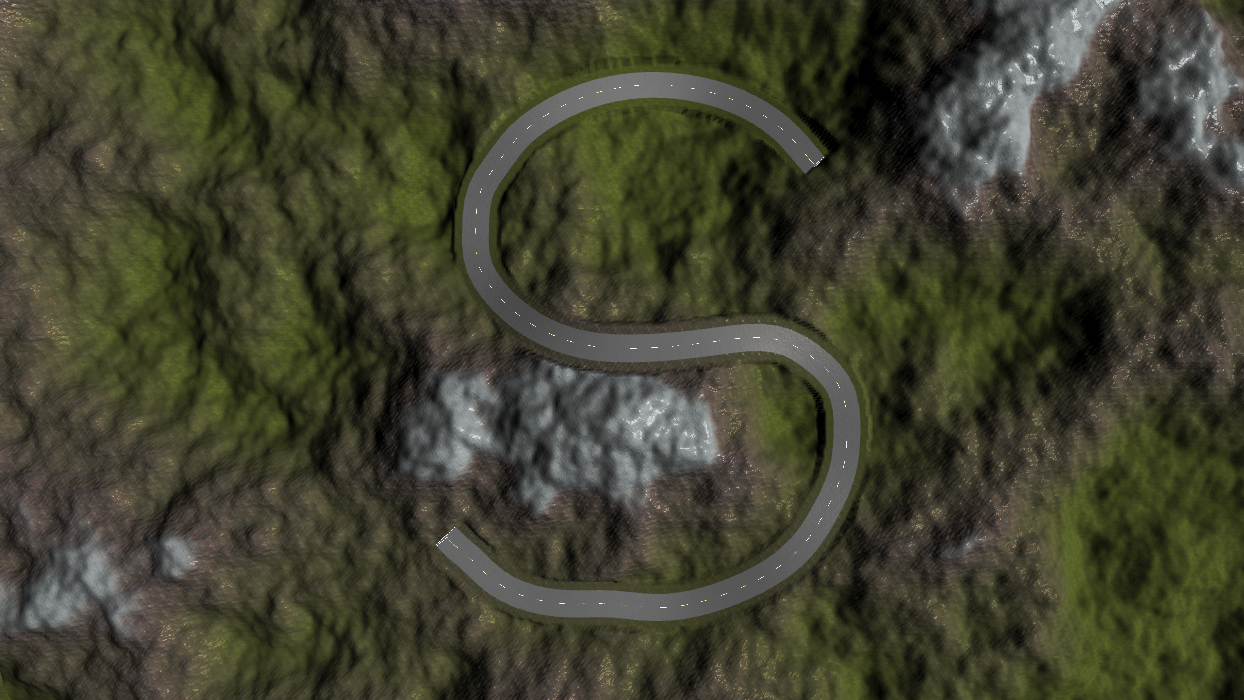
\includegraphics[width=0.4\linewidth]{thesis/related/applegate2.png}
 \caption{The road sketching approach from Applegate et al. \cite{applegate2011sketch}. }
 \label{fig:applegate}
\end{figure}

Applegate et al. \cite{applegate2011sketch} have a sketch based system for highway design which is illustrated in Figure \ref{fig:applegate}. Their tool is guided by input sketches and a combination of prioritized constraints, including the curvature of roads, their inclination, and the volume of underlying terrain that is displaced. The rivers in my proposed solution are sketched in a similar way to this highway sketching method by projecting the sketches onto the terrain and then creating geometry and making terrain modifications along the path the user has sketched. In developing my proposed approach I have taken inspiration from many of the techniques that were presented in this chapter. In the next chapter I present all the techniques which I have employed to create my proposed approach.


\section{Approach}


I employ a sketch-based input that is projected onto a transparent cube. Layered geological structures are often sketched in a cube, and I therefore propose to mimic this technique for the sketching interface. The user can rotate around the cube and sketch on the four vertical faces of the cube. On the faces the user sketches the outlines of a surface that will be the top boundary of one of the layer volumes. The surface is then interpolated between the sketched outline. In geology, a surface the is called a horizon. The horizon is also what separates two layers stacked on top of each other. I therefore use the top horizons of previously drawn layers as the bottom boundary of new layers. The user can thus create a stack of layers by adding the layers from bottom to top.

In order to change and model details on the layers, I propose methods for drawing further structure features such as mountains, rivers, valleys and deposits. The user can create ridges, rivers and valleys by sketching on the layers. Separate algorithms for each of the features will then modify the layer surface on which it was drawn. The features the user sketches are positioned on the 2D manifold of the surface it was sketched on, such that a change in the underlying layers representation can be made without having to redraw or manually reposition all the features that exist on that layer. Deposits are created by a procedure that distributes material from the point where the river meets the sea. The material is distributed by a volume preserving diffusion algorithm that considers the topology of the underlying layer surface to create a plausible flow of material from the river.

\section{Evaluation}
The results in the previous section indicate that the approach suggested has a potential use in illustrating geological phenomena. As Figure \ref{fig:sketchRepro} shows, even after a short introduction of about 10 minutes, test subjects from the geologic field were able to draw figures resembling the sketch they were trying to reproduce. Figure \ref{fig:sketchRepro2} shows that a person familiar with the program can create more detailed sketches, and the ray-traced image indicates the possibility of using the created models in further applications. Exporting could thus allow more detailed features to be added to the models at a later stage by people with such expertize.

Figure \ref{fig:glacier} and \ref{fig:subduction} shows that reproduction of some illustrations of geological educational material is already possible with this approach. Some details are missing, but the most important processes are captured. With a little more development of the approach, these examples should be perfectly reproducible to the extent that all the important features are captured in a reproduction.

When the approach gains more maturity, I expect it or some similar approach could become the standard way to illustrate geological phenomena by students, teachers and researchers. I base this expectation on the fact that all these drawings were made in a matter of minutes. Subjects from the user study indicated that they use considerable time creating such sketches by 2D methods and that they believed it would save them time. Subjects in this study were all students, but I would expect also experienced geologists sometimes use considerable time when creating conceptual geological illustrations and that they  could all benefit from the new modeling approach.

The user study also sheds some more light on what aspects of the approach work and in what direction any further work might consider going. The subjects responded very positively to the approach, although they indicated that further development is needed to make it useful in many scenarios they need to illustrate. According to the study, the chosen input method for creating a surface makes it possible to draw simple surfaces quickly compared to what subjects draw on paper. However, as betrayed by the glacier reproduction attempt (Figure \ref{fig:glacier}), the algorithm that interpolates the lines drawn works in such a way that it will favor structures that manifest themselves along the interpolation direction. Similar structures could be made in that instance by the valley feature, but it can be frustrating for a user to draw the same type of features in one case and another in other cases. Other features like rivers, ridges and sketches were all described as easy to use. However, the valleys and ridges 
could benefit from 
more control over depth and width respectively. 

Deposits are a feature that shows how a procedural approach can be combined with the sketching approach for creating surfaces. It is the last feature that was included, and will need more development to show its real potential. Subjects remarked on some bugs, and requested more features regarding the deposits however, so in their eyes it presumably can also be useful to illustrate deposits in the proposed way. 

During the development of the approach, work was conducted in an experimental fashion. I would try out different approaches, and decide which one worked best based on trying it, often together with Marie. After a while I decided I needed some discussion and collaboration with people from the geologic field to continue. This was very helpful during the development phase in order to get direction and focus where my own experience and knowledge about geology was not sufficient. I suspect that involving geologists from an even earlier point could have helped the process. Even in questions not pertaining directly to geology, it was helpful to get input from people not from the computer science field. They were not familiar with the internals of my particular implementation and way of thinking, and would therefore mention problems that I would not notice. Several usability issues were ironed out this way.

All in all the project has been a success. I could definitely have used more time to add numerous features and refining the ones that are there today, but the results show that the idea of drawing in a box was a good one and that the approach could be used, with further development, by geologists to make many of their illustrations.


%- learning\\
%- usability
% -- (focus on expressiveness) -- \\
%- How well problem was solved\\
%- Where it will be used \\
%- Discussion

\section{Further work}
Of the difficulties I found with modeling geology in a rapid way is to make all the different features interact correctly, while keeping the input on an abstract level to keep the modeling simple. There are many different processes that geologists need to model. There is a trade off between the amount of time needed to model, and the possibilities the modeling approach offers. The real challenge is to minimize the negative effects of this trade off while incorporating more features.

I would really like to develop an intuitive approach for making fault structures in the layers. Faults are definitely a needed feature, and by my own understanding of geologist's needs, how often faults are encountered and based on test subjects feedback, a feature for sketching faults would be the natural next step for further research. I think an easy way to input such faults could be to let the user sketch curves on each horizon where the intersection of faults and layers should be. An interpolation of these curves would then create a surface representing the fault. The user could then indicate by sketching on this surface how far the layers involved have faulted. Finally an algorithm would be needed that could morph the layers and any features already drawn on them.

Another feature I would like to see, is the ability to combine several cubes into a bigger scene. This would require some means of using what has already been sketched on one cube as a starting point for adjacent cubes. In order to not impose too much work on the user, the surface creation algorithm would need modification to ensure continuity of surfaces across cubes. I think that conducting further research into using the Inverse Distance Weighing interpolation approach, could help with this since it could take into account the points on both adjacent cubes in the weighting. The Discrete Smooth Interpolation developed by Mallet \cite{mallet1992gocad} would also be interesting to explore for allowing smooth transition between the cubes. The ability to change a cubes height, width and depth is another possible feature that could be useful. To make this cube change work together with the multiple cubes all cubes could be restricted to the same size, so they will align properly.

There is also a number of possible improvements on the features that are already included. The river width control can today be a bit difficult to use if the user wants to create narrow rivers. This difficulty could perhaps be removed if there was a way to change the width across the entire river in one go, instead of having to carefully sketch along the entire rivers length. Ridges could benefit from some method of sketching the width along the length of the ridge. I think both depth and width control could be achieved by additional sketching surfaces. If the user could sketch the profile in of a river, valley or ridge orthogonal to the direction of the initially sketched base line, I think this would be sufficient to create many desirable versions of such features. To make this feature even more powerful, it could be possible to input several such profiles along the length of the feature, and the profile could be interpolated between them.

To make deposits a more powerful feature, I would make them into fully fledged layers. By this I mean that it should be possible to modify them in all the same ways as the sketched layers in the cube. The procedure that creates the deposits could also have more parameters, like how far it will flow, how much material is transported, how fast the river flows, etc. It could take into account the possibility of the river stream carrying different sized particles at the same time, thus depositing them in different regions. The flow speed of the river could be calculated based on the terrain slope. The amount of deposited material would be dependent on several factors possibly outside the sketch, such as terrain material and length of river. Deposits could also benefit from more control over the shape.

Many of the illustrations could benefit from a feature that allowed painting on the surfaces of the sketch like Natali et al. \cite{natalirapid}, and by creating billboards such as Cohen \cite{cohen2000harold} suggests. Painting on the surfaces would for example allow the illustration of subduction of oceanic plates sketch in Figure \ref{fig:subduction} to be completely reproduced. A billboard feature would also allow geologist to input context giving features such as vegetation and animal life, plumes of smoke from volcanoes, etc. Such details can be seen in many of the illustrations in \secref{sec:geology}. With a painting and billboards feature artistic users could input details that would improve the visual appearance of the illustration. I would also like to see a texturing feature similar to what Natali et al. proposes where textures by default follow the layer structure, but the user can sketch to override its direction and deformation to illustrate details of a layers internal structure. Another way 
to add a more realistic look for the horizon surfaces could be achieved through a fractal noise method.

If implementing any of these features it is important to focus on the usability and ease of use. In that respect I would continue to involve users from the geologic field. One of the characteristics test users have commented was the ease of use of the features and of creating sketches in this approach. If it would become more difficult to use, they might prefer to draw illustrations by hand. It should preferably not become more complicated to model the scenes that are already possible to create. New features should simply add possibilities that are as easy to use as the rest.


\section{Conclusion}
This thesis started by explaining how geologists have a use for an application that lets them create simple models that lets them illustrate their thoughts amongst themselves. In education and literature such illustrative tools are also useful. A goal was stated: to create an approach for rapid and easy sketching of geologic structures in 3D. The relevant geological background was explained and the state of the art for rapid sketching of geology was described. An approach for a tool for rapid modeling of geologic structures was given and how it was developed was explained in detail. This approach explained was mostly based on sketch input, but also incorporated a procedural method to explore the possibility of combination of these two rapid modeling metaphors.

Screenshots of geologic scenes that can be modeled using the currently implemented algorithms were given. A user study showed that such a tool is indeed highly interesting for the target group of people. The approach developed has some merit to it according to this user study, although further development is still needed for it to be useful in more than a few simple cases. However, the subjects of the study indicated their belief that the approach has potential. The input methods were described as easy to use, although most of the features need further development to enable sketching of desired geological scenarios. Even in the state the implemented solution is in now though, some users expressed a possibility for applying the solution in real world situations.

Finally some thoughts for further research were discussed what I think would be the natural next steps to improve this approach. Particularly, fault structures are a feature that occurs in many geological illustrations. When developing new features, focus should be given to what potential users are comfortable with and to preserving the ease of use that the approach already has.

I expect that when this approach gains more maturity, or similar approaches are developed to maturity, they could become the standard way to illustrate geological phenomena by students, teachers and researchers, based on the illustrated results and user study. Although further research and development is still needed to enable more geological scenarios to be illustrated, the user feedback indicated that the approach is intuitive to use and enables rapid illustration of certain geological scenarios. The goal of the thesis, to create an approach that can be used for making rapid 3D illustrations for geologic uses, has thus been reached.


 %%% The bibliography
\bibliographystyle{plain}
\bibliography{shortPaper}

\end{document}

\endinput
%%
%% End of file `cescgsmpl.tex'.
